We decided to use pre-traind VGG16 model, without its top two layers.\\

{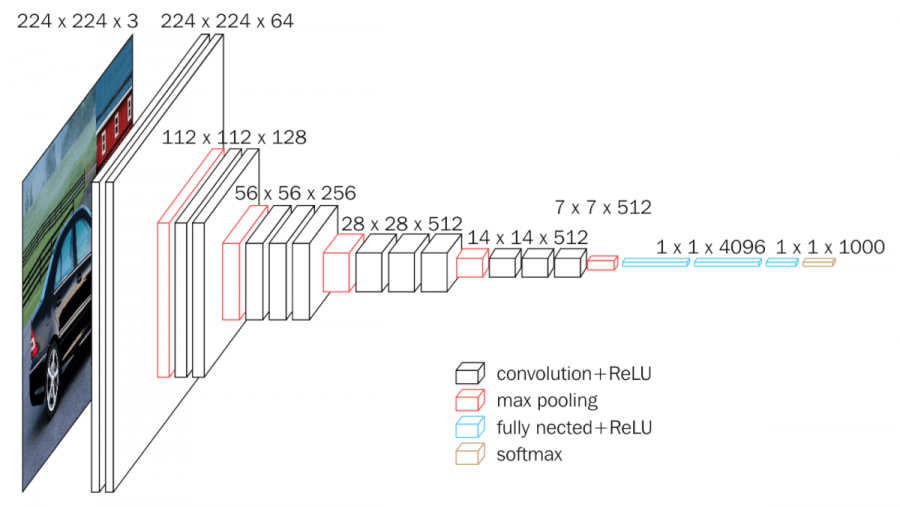
\includegraphics[scale=0.5]{./images/vgg16.png}} \\

VGG16 is a convolutional neural network model proposed by K. Simonyan and A. Zisserman
from the University of Oxford in the paper “Very Deep Convolutional Networks
for Large-Scale Image Recognition”. The model achieves 92.7%
top-5 test accuracy in ImageNet, which is a dataset of over 14 million
images belonging to 1000 classes. It was one of the famous model submitted
to ILSVRC-2014. It makes the improvement over AlexNet by replacing large
kernel-sized filters (11 and 5 in the first and second convolutional layer,
respectively) with multiple 3×3 kernel-sized filters one after another. VGG16
was trained for weeks and was using NVIDIA Titan Black GPU’s.

In Keras it's really easy to implemnt this model and freeze layers to non-trainable (In code in "Implementaion" section)
Our VGG model looks lika this:\\

{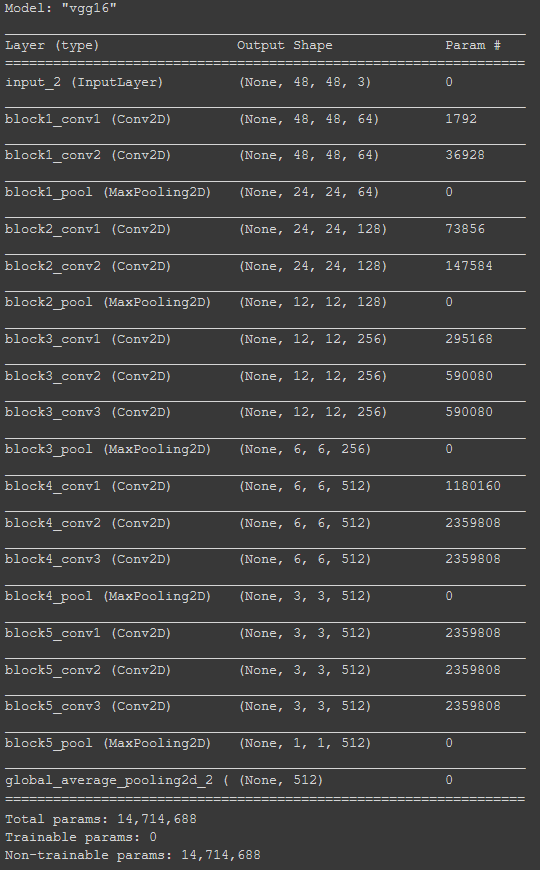
\includegraphics[scale=0.5]{./images/vggNT.png}} \\

